\documentclass[a4paper]{article}

\def\npart {III}
\def\nterm {Michaelmas}
\def\nyear {2017}
\def\nlecturer {B. Bollobas}
\def\ncourse {Combinatorics}

% Imports
\ifx \nextra \undefined
  \usepackage[pdftex,
    hidelinks,
    pdfauthor={Dexter Chua},
    pdfsubject={Cambridge Maths Notes: Part \npart\ - \ncourse},
    pdftitle={Part \npart\ - \ncourse},
  pdfkeywords={Cambridge Mathematics Maths Math \npart\ \nterm\ \nyear\ \ncourse}]{hyperref}
  \title{Part \npart\ - \ncourse}
\else
  \usepackage[pdftex,
    hidelinks,
    pdfauthor={Dexter Chua},
    pdfsubject={Cambridge Maths Notes: Part \npart\ - \ncourse\ (\nextra)},
    pdftitle={Part \npart\ - \ncourse\ (\nextra)},
  pdfkeywords={Cambridge Mathematics Maths Math \npart\ \nterm\ \nyear\ \ncourse\ \nextra}]{hyperref}

  \title{Part \npart\ - \ncourse \\ {\Large \nextra}}
\fi

\author{Lectured by \nlecturer \\\small Notes taken by Dexter Chua}
\date{\nterm\ \nyear}

\usepackage{alltt}
\usepackage{amsfonts}
\usepackage{amsmath}
\usepackage{amssymb}
\usepackage{amsthm}
\usepackage{booktabs}
\usepackage{caption}
\usepackage{enumitem}
\usepackage{fancyhdr}
\usepackage{graphicx}
\usepackage{mathtools}
\usepackage{microtype}
\usepackage{multirow}
\usepackage{pdflscape}
\usepackage{pgfplots}
\usepackage{siunitx}
\usepackage{tabularx}
\usepackage{tikz}
\usepackage{tkz-euclide}
\usepackage[normalem]{ulem}
\usepackage[all]{xy}

\pgfplotsset{compat=1.12}

\pagestyle{fancyplain}
\lhead{\emph{\nouppercase{\leftmark}}}
\ifx \nextra \undefined
  \rhead{
    \ifnum\thepage=1
    \else
      \npart\ \ncourse
    \fi}
\else
  \rhead{
    \ifnum\thepage=1
    \else
      \npart\ \ncourse\ (\nextra)
    \fi}
\fi
\usetikzlibrary{arrows}
\usetikzlibrary{decorations.markings}
\usetikzlibrary{decorations.pathmorphing}
\usetikzlibrary{positioning}
\usetikzlibrary{fadings}
\usetikzlibrary{intersections}
\usetikzlibrary{cd}

\newcommand*{\Cdot}{\raisebox{-0.25ex}{\scalebox{1.5}{$\cdot$}}}
\newcommand {\pd}[2][ ]{
  \ifx #1 { }
    \frac{\partial}{\partial #2}
  \else
    \frac{\partial^{#1}}{\partial #2^{#1}}
  \fi
}

% Theorems
\theoremstyle{definition}
\newtheorem*{aim}{Aim}
\newtheorem*{axiom}{Axiom}
\newtheorem*{claim}{Claim}
\newtheorem*{cor}{Corollary}
\newtheorem*{defi}{Definition}
\newtheorem*{eg}{Example}
\newtheorem*{fact}{Fact}
\newtheorem*{law}{Law}
\newtheorem*{lemma}{Lemma}
\newtheorem*{notation}{Notation}
\newtheorem*{prop}{Proposition}
\newtheorem*{thm}{Theorem}

\renewcommand{\labelitemi}{--}
\renewcommand{\labelitemii}{$\circ$}
\renewcommand{\labelenumi}{(\roman{*})}

\let\stdsection\section
\renewcommand\section{\newpage\stdsection}

% Strike through
\def\st{\bgroup \ULdepth=-.55ex \ULset}

% Maths symbols
\newcommand{\bra}{\langle}
\newcommand{\ket}{\rangle}

\newcommand{\N}{\mathbb{N}}
\newcommand{\Z}{\mathbb{Z}}
\newcommand{\Q}{\mathbb{Q}}
\renewcommand{\H}{\mathbb{H}}
\newcommand{\R}{\mathbb{R}}
\newcommand{\C}{\mathbb{C}}
\newcommand{\Prob}{\mathbb{P}}
\renewcommand{\P}{\mathbb{P}}
\newcommand{\E}{\mathbb{E}}
\newcommand{\F}{\mathbb{F}}
\newcommand{\cU}{\mathcal{U}}
\newcommand{\RP}{\mathbb{RP}}
\newcommand{\CP}{\mathbb{CP}}

\newcommand{\ph}{\,\cdot\,}

\DeclareMathOperator{\sech}{sech}
\DeclareMathOperator{\cosech}{cosech}
\DeclareMathOperator{\cosec}{cosec}

\DeclareMathOperator{\covol}{covol}
\DeclareMathOperator{\vol}{vol}

\let\Im\relax
\let\Re\relax
\DeclareMathOperator{\Im}{Im}
\DeclareMathOperator{\Re}{Re}
\DeclareMathOperator{\im}{im}
\DeclareMathOperator{\image}{image}
\DeclareMathOperator{\Ann}{Ann}

\DeclareMathOperator*{\res}{res}
\DeclareMathOperator{\Res}{Res}
\DeclareMathOperator{\Ind}{Ind}

\DeclareMathOperator{\tr}{tr}
\DeclareMathOperator{\diag}{diag}
\DeclareMathOperator{\rank}{rank}
\DeclareMathOperator{\card}{card}
\DeclareMathOperator{\spn}{span}
\DeclareMathOperator{\adj}{adj}

\DeclareMathOperator{\erf}{erf}
\DeclareMathOperator{\erfc}{erfc}

\DeclareMathOperator{\ord}{ord}
\DeclareMathOperator{\Sym}{Sym}

\DeclareMathOperator{\sgn}{sgn}
\DeclareMathOperator{\orb}{orb}
\DeclareMathOperator{\stab}{stab}
\DeclareMathOperator{\ccl}{ccl}

\DeclareMathOperator{\lcm}{lcm}
\DeclareMathOperator{\hcf}{hcf}

\DeclareMathOperator{\Int}{Int}
\DeclareMathOperator{\id}{id}

\DeclareMathOperator{\betaD}{beta}
\DeclareMathOperator{\gammaD}{gamma}
\DeclareMathOperator{\Poisson}{Poisson}
\DeclareMathOperator{\binomial}{binomial}
\DeclareMathOperator{\multinomial}{multinomial}
\DeclareMathOperator{\Bernoulli}{Bernoulli}
\DeclareMathOperator{\like}{like}

\DeclareMathOperator{\var}{var}
\DeclareMathOperator{\cov}{cov}
\DeclareMathOperator{\bias}{bias}
\DeclareMathOperator{\mse}{mse}
\DeclareMathOperator{\corr}{corr}

\DeclareMathOperator{\otp}{otp}
\DeclareMathOperator{\dom}{dom}

\DeclareMathOperator{\Root}{Root}
\DeclareMathOperator{\supp}{supp}
\DeclareMathOperator{\rel}{rel}
\DeclareMathOperator{\Hom}{Hom}
\DeclareMathOperator{\Aut}{Aut}
\DeclareMathOperator{\Gal}{Gal}
\DeclareMathOperator{\Mat}{Mat}
\DeclareMathOperator{\End}{End}
\DeclareMathOperator{\Char}{char}
\DeclareMathOperator{\ev}{ev}
\DeclareMathOperator{\St}{St}
\DeclareMathOperator{\Lk}{Lk}
\DeclareMathOperator{\disc}{disc}
\DeclareMathOperator{\Isom}{Isom}
\DeclareMathOperator{\length}{length}
\DeclareMathOperator{\energy}{energy}
\DeclareMathOperator{\area}{area}
\DeclareMathOperator{\Syl}{Syl}
\DeclareMathOperator{\cl}{cl}
\DeclareMathOperator{\fix}{fix}

\newcommand{\GL}{\mathrm{GL}}
\newcommand{\SL}{\mathrm{SL}}
\newcommand{\PGL}{\mathrm{PGL}}
\newcommand{\PSL}{\mathrm{PSL}}
\newcommand{\PSU}{\mathrm{PSU}}
\newcommand{\Or}{\mathrm{O}}
\newcommand{\SO}{\mathrm{SO}}
\newcommand{\U}{\mathrm{U}}
\newcommand{\SU}{\mathrm{SU}}

\renewcommand{\d}{\mathrm{d}}
\newcommand{\D}{\mathrm{D}}

\tikzset{->/.style = {decoration={markings,
                                  mark=at position 1 with {\arrow[scale=2]{latex'}}},
                      postaction={decorate}}}
\tikzset{<-/.style = {decoration={markings,
                                  mark=at position 0 with {\arrowreversed[scale=2]{latex'}}},
                      postaction={decorate}}}
\tikzset{<->/.style = {decoration={markings,
                                   mark=at position 0 with {\arrowreversed[scale=2]{latex'}},
                                   mark=at position 1 with {\arrow[scale=2]{latex'}}},
                       postaction={decorate}}}
\tikzset{->-/.style = {decoration={markings,
                                   mark=at position #1 with {\arrow[scale=2]{latex'}}},
                       postaction={decorate}}}
\tikzset{-<-/.style = {decoration={markings,
                                   mark=at position #1 with {\arrowreversed[scale=2]{latex'}}},
                       postaction={decorate}}}

\tikzset{circ/.style = {fill, circle, inner sep = 0, minimum size = 3}}
\tikzset{mstate/.style={circle, draw, blue, text=black, minimum width=0.7cm}}

\definecolor{mblue}{rgb}{0.2, 0.3, 0.8}
\definecolor{morange}{rgb}{1, 0.5, 0}
\definecolor{mgreen}{rgb}{0.1, 0.4, 0.2}
\definecolor{mred}{rgb}{0.5, 0, 0}

\def\drawcirculararc(#1,#2)(#3,#4)(#5,#6){%
    \pgfmathsetmacro\cA{(#1*#1+#2*#2-#3*#3-#4*#4)/2}%
    \pgfmathsetmacro\cB{(#1*#1+#2*#2-#5*#5-#6*#6)/2}%
    \pgfmathsetmacro\cy{(\cB*(#1-#3)-\cA*(#1-#5))/%
                        ((#2-#6)*(#1-#3)-(#2-#4)*(#1-#5))}%
    \pgfmathsetmacro\cx{(\cA-\cy*(#2-#4))/(#1-#3)}%
    \pgfmathsetmacro\cr{sqrt((#1-\cx)*(#1-\cx)+(#2-\cy)*(#2-\cy))}%
    \pgfmathsetmacro\cA{atan2(#2-\cy,#1-\cx)}%
    \pgfmathsetmacro\cB{atan2(#6-\cy,#5-\cx)}%
    \pgfmathparse{\cB<\cA}%
    \ifnum\pgfmathresult=1
        \pgfmathsetmacro\cB{\cB+360}%
    \fi
    \draw (#1,#2) arc (\cA:\cB:\cr);%
}
\newcommand\getCoord[3]{\newdimen{#1}\newdimen{#2}\pgfextractx{#1}{\pgfpointanchor{#3}{center}}\pgfextracty{#2}{\pgfpointanchor{#3}{center}}}

\def\Xint#1{\mathchoice
   {\XXint\displaystyle\textstyle{#1}}%
   {\XXint\textstyle\scriptstyle{#1}}%
   {\XXint\scriptstyle\scriptscriptstyle{#1}}%
   {\XXint\scriptscriptstyle\scriptscriptstyle{#1}}%
   \!\int}
\def\XXint#1#2#3{{\setbox0=\hbox{$#1{#2#3}{\int}$}
     \vcenter{\hbox{$#2#3$}}\kern-.5\wd0}}
\def\ddashint{\Xint=}
\def\dashint{\Xint-}


\begin{document}
\maketitle
{\small
\setlength{\parindent}{0em}
\setlength{\parskip}{1em}

What can one say about a collection of subsets of a finite set satisfying certain conditions in terms of containment, intersection and union? In the past fifty years or so, a good many fundamental results have been proved about such questions: in the course we shall present a selection of these results and their applications, with emphasis on the use of algebraic and probabilistic arguments.

The topics to be covered are likely to include the following:
\begin{itemize}
 \item The de Bruijn--Erd\"os theorem and its extensions.
 \item The Graham--Pollak theorem and its extensions.
 \item The theorems of Sperner, EKR, LYMB, Katona, Frankl and F\"uredi. % check Furedi
 \item Isoperimetric inequalities: Kruskal--Katona, Harper, Bernstein, BTBT, and their applications.
 \item Correlation inequalities, including those of Harris, van den Berg and Kesten, and the Four Functions Inequality.
 \item Alon's Combinatorial Nullstellensatz and its applications.
 \item LLLL and its applications.
\end{itemize}

\subsubsection*{Pre-requisites}
The main requirement is mathematical maturity, but familiarity with the basic graph theory course in Part II would be helpful.
}
\tableofcontents

\section{Hall's theorem}
We shall begin with a discussion of Hall's theorem. Ideally, you've already met it in IID Graph Theory. We shall see that this has some interesting combinatorial implications. We shall start with some rather elementary definitions.

\begin{defi}[Bipartite graph]\index{bipartite graph}
  We say $G = (X, Y; E)$ is a \emph{bipartite graph} with bipartition $X$ and $Y$ if $(X \coprod Y, E)$ is a graph such that every edge is between a vertex in $X$ and a vertex in $Y$.

  We say such a bipartite graph is \term{$(k, \ell)$-regular} if every vertex in $X$ has degree $k$ and every vertex in $Y$ has degree $\ell$.
\end{defi}

\begin{defi}[Complete matching]\index{complete matching}
  Let $G = (X, Y; E)$ be a bipartite graph with bipartition $X$ and $Y$. A \emph{complete matching} from $X$ to $Y$ is an injection $f: X \to Y$ such that $x\, f(x)$ is an edge for every $x \in X$.
\end{defi}

Hall's theorem gives us a necessary and sufficient condition for the existence of a complete matching. Let's try to first come up with a necessary condition. If there is a complete matching, then for any subset $S \subseteq X$, we certainly have $|\Gamma(S)| \geq |S|$, where \term{$\Gamma(S)$} is the set of neighbours of $S$. It turns out this is also sufficient.

\begin{thm}[Hall, 1935]\index{Hall's theorem}
  A bipartite graph $G = (X, Y; E)$ has a complete matching from $X$ to $Y$ if and only if $|\Gamma(S)| \geq |S|$ for all $S \subseteq X$.
\end{thm}
This condition is known as \term{Hall's condition}.

\begin{proof}
  We may assume $G$ is edge-minimal satisfying Hall's condition. We show that $G$ is a complete matching from $X$ to $Y$. For $G$ to be a complete matching, we need the following two properties:
  \begin{enumerate}
    \item Every vertex in $X$ has degree $1$
    \item Every vertex in $Y$ has degree $0$ or $1$.
  \end{enumerate}

  We first examine the second condition. Suppose $y \in Y$ is such that there exists edges $x_1 y, x_2 y \in E$. Then the minimality of $G$ implies there are sets, $X_1, X_2 \subseteq X$ such that $x_i \in X_i$ such that $|\Gamma(X_i)| = |X_i|$ and $x_i$ is the only neighbour of $y$ in $X_i$.

  Now consider the set $X_1 \cap X_2$. We know $\Gamma(X_1 \cap X_2) \subseteq \Gamma(X_1) \cap \Gamma(X_2)$. Moreover, this is strict, as $y$ is in the RHS but not the LHS. So we have
  \[
    \Gamma(X_1 \cap X_2) \leq |\Gamma(X_i) \cap \Gamma(X_2)| - 1.
  \]
  But also
  \begin{align*}
    |X_1 \cap X_2| &\leq |\Gamma(X_1 \cap X_2)|\\
    &\leq |\Gamma(X_1) \cap \Gamma(X_2)| - 1 \\
    &= |\Gamma(X_1)| + |\Gamma(X_2)| - |\Gamma(X_1) \cup \Gamma(X_2)| - 1\\
    &= |X_1| + |X_2| - |\Gamma(X_1\cup X_2)| - 1\\
    &\leq |X_1| + |X_2| - |X_1 \cup X_2| - 1\\
    &= |X_1 \cap X_2| - 1,
  \end{align*}
  which contradicts Hall's condition.

  One then sees that the first condition is also satisfied --- if $x \in X$ is a vertex, then the degree of $x$ certainly cannot be $0$, or else $|\Gamma(\{x\})| < |\{x\}|$, and we see that $d(x)$ cannot be $>1$ or else we can just remove an edge from $x$ without violating Hall's condition.
\end{proof}

We shall now describe some consequences of Hall's theorem. They will be rather straightforward applications, but we shall later see they have some interesting consequences.

Let $\mathcal{A} = \{A_1, \ldots, A_m\}$ be a set system. All sets are finite. A set of \term{distinct representatives} of $\mathcal{A}$ is a set $\{a_1, \ldots a_m\}$ of distinct elements $a_i \in A_i$.

Under what condition do we have a set of distinct representatives? If we have one, then for any $I \subseteq [m] = \{1, 2, \ldots, m\}$, we have
\[
  \left|\bigcup_{i \in I} A_i \right| \geq |I|.
\]
We might hope this is sufficient.
\begin{thm}
  $\mathcal{A}$ has a set of distinct representatives iff for all $\mathcal{B} \subseteq \mathcal{A}$, we have
  \[
    \left|\bigcup_{B \in \mathcal{B}} B\right| \geq |\mathcal{B}|.
  \]
\end{thm}

This is an immediate consequence of Hall's theorem.

\begin{proof}
  Define a bipartite graph as follows --- we let $X = \mathcal{A}$, and $Y = \bigcup_{i \in [m]} A_i$. Then draw an edge from $x$ to $A_i$ if $x \in A_i$. Then there is a complete matching of this graph iff $\mathcal{A}$ has a set of distinct representations, and the condition in the theorem is exactly Hall's condition. So we are done by Hall's theorem.
\end{proof}

\begin{thm}
  Let $G = (X, Y; E)$ be a bipartite graph such that $d(x) \geq d(y)$ for all $x \in X$ and $y \in Y$. Then there is a complete matching from $X$ to $Y$.
\end{thm}

\begin{proof}
  Let $d$ be such that $d(x) \geq d \geq d(y)$ for all $x \in X$ and $y \in Y$. For $S \subseteq X$ and $T \subseteq Y$, we let $e(S, T)$ be the number of edges between $S$ and $T$. Let $S \subseteq X$, and $T = \Gamma(S)$. Then we have
  \[
    e(S, T) = \sum_{x \in S} d(x) \geq d |S|,
  \]
  but on the other hand, we have
  \[
    e(S, T) \leq \sum_{y \in T} d(y) \leq d |T|.
  \]
  So we find that $|T| \geq |S|$. So Hall's condition is satisfied.
\end{proof}

\begin{cor}
  If $G = (X, Y; E)$ is a $(k, \ell)$-regular bipartite graph with $1 \leq \ell \leq k$, then there is a complete matching from $X$ to $Y$.
\end{cor}

\begin{defi}[Biregular graph]\index{biregular graph}
  A graph is \emph{biregular} if it is bipartite and $(k,\ell)$-regular for some $k, \ell \geq 1$.
\end{defi}
Then by really basic counting arguments, we hahve
\[
  |E| = |X| k = |Y| \ell,
\]
and so
\[
  \frac{k}{\ell} = \frac{|Y|}{|X|}.
\]
\begin{thm}
  Let $G = (X, Y; E)$ be biregular and $A \subseteq X$. Then
  \[
    \frac{|\Gamma(A)|}{|Y|}\geq \frac{|A|}{|X|}.
  \]
\end{thm}

\begin{proof}
  Suppose $G$ is $(k, \ell)$-regular. The idea is to look at the subgraph containing $A$ and $\Gamma(A)$. Then
  \[
    k|A| = e(A, \Gamma(A)) \leq \ell |\Gamma(A)|.
  \]
  Thus
  \[
    \frac{|\Gamma(A)|}{|Y|} \geq \frac{k|A|}{\ell |Y|} = \frac{|A|}{|X|}.
  \]
\end{proof}
Briefly, this says biregular graphs ``expand''.

\begin{cor}
  Let $G = (X, Y; E)$ be biregular and let $|X| \leq |Y|$. Then there is a complete matching of $X$ into $Y$.
\end{cor}

\begin{notation}\index{$X^{(r)}$}\index{$X^{(\leq r)}$}\index{$X^{\geq r}$}
  Given a set $X$, we write $X^{(r)}$ for the set of all subsets of $X$ with $r$ elements, and similarly for $X^{(\geq r)}$ and $X^{(\leq r)}$.
\end{notation}

If $|X| = n$, then $|X^{(r)}| = \binom{n}{r}$.

Now given a set $X$ and two numbers $r < s$, we can construct a biregular graph $(X^{(r)}, X^{(s)}; E)$, where $A \in X^{(r)}$ is joined to $B \in X^{(s)}$ if $A \subseteq B$.

\begin{cor}
  Let $1 \leq r < s \leq |X| = n$. Suppose $|\frac{n}{2} -r | \geq |\frac{n}{2} - s|$. Then there exists an injection $f: X^{(r)} \to X^{(s)}$ such that $A \subseteq f(A)$ for all $A \in X^{(r)}$.

  if $|n/2 - r| \leq |n/2 - s|$, then there exists an injection $g: X^{(s)} \to X^{(r)}$ such that $A \supseteq g(A)$ for all $A \in X^{(s)}$.
\end{cor}

\begin{proof}
  Note that $|n/2 - r| \leq |n/2 - s|$ iff $\binom{n}{r} \geq \binom{n}{s}$.
\end{proof}

\section{Sperner systems}
We'll consider posets $\mathcal{P} = (S, <)$.
\begin{defi}[Chain]\index{chain}
  A subset $C \subseteq S$ of a poset is a \emph{chain} if any two of its elements are comparable.
\end{defi}

\begin{defi}[Anti-chain]\index{anti-chain}
  A subset $A \subseteq S$ is an \emph{anti-chain} if no two of its elements are comparable.
\end{defi}

Given a set $X$, we will write $\mathcal{P}(X)$ for the power set of $X$, thought of as a Boolean lattice. This is a poset by saying $A < B$ if $A \subsetneq B$.

\begin{defi}[Graded poest]\index{graded poset}
  We say $\mathcal{P} = (S, <$ is a \emph{graded poset} if we can write $S$ as a disjoint union
  \[
    S = \coprod_{i = 0}^n S_i % union with dot on top
  \]
  such that
  \begin{itemize}
    \item $S_i$ is an anti-chain; and
    \item $x < y$ iff there exists elements $x = z_i < z_{i + 1} < \cdots < z_j = y$ such that $z_h \in S_h$.
  \end{itemize}
\end{defi}
\begin{eg}
  If $X$ is a set, $\mathcal{P}(X)$ is an anti-chain with $X_i = X^{(i)}$.
\end{eg}
\begin{thm}[Sperner, 1928]
  For $|X| = n$, the maximal size of an antichain in $\mathcal{P}(X)$ is $\binom{n}{\lfloor n/2\rfloor}$, witnessed by $X^{\lfloor n/2\rfloor}$.
\end{thm}

\begin{proof}
  If $\mathcal{C}$ is a chain and $\mathcal{A}$ is an antichain, then $|\mathcal{A} \cap \mathcal{C}| \leq 1$. So it suffices to partition $\mathcal{P}(X)$ into
  \[
    m = \max_{k} \binom{n}{k} = \binom{n}{\lfloor n/2\rfloor} = \binom{n}{\lceil n/2 \rceil}
  \]
  many chains. We can do so using the injections constructed at the end of the previous section.

  Indeed, we can use them to partition $X^{(\geq \lfloor n/2 \rfloor)}$ into $m$ chains with each ending in $X^{(\lfloor n/2\rfloor)}$, and similarly, we can partition $X^{(\leq \lfloor n/2\rfloor)}$ into $m$ chains with each chain ending in $X^{(\lfloor n/2\rfloor)}$. Then glue them together.

  % insert picture

\end{proof}

\begin{thm}[LYM inequality]
  Let $\mathcal{A}$ be an antichain in $\mathcal{P}(X)$ with $|X| = n$. Then
  \[
    \sum_{r = 0}^n \frac{|\mathcal{A} \cap X^{(r)}|}{\binom{n}{r}} \leq 1.
  \]
  In particular, $|\mathcal{A}| \leq \max_r \binom{n}{r} = \binom{n}{\lfloor n\rfloor}$, as we already know.
\end{thm}

\begin{proof}
  A chain $C_0 \subseteq C_1 \subseteq \cdots \subseteq C_m$ is maximal if it has $n + 1$ elements. Moreover, there is a bijection by a maximal chains with maps $[n] \to X$, sending $i$ to the element in $C_i \setminus C_{i - 1}$. Therefore there are $n!$ maximal chains.

  For ever maximal chain $\mathcal{C}$, we have $|\mathcal{C} \cap \mathcal{A}| \leq 1$. Moreover, every set of $k$ elements appears in $k! (n - k)!$ maximal chains. So
  \[
    \sum_{A \in \mathcal{A}} |A|! (n - |A|)! \leq n!.
  \]
  Then the result follows.
\end{proof}

\begin{defi}[Shadow]\index{shadow}
  Given $A \subseteq S_i$, the \emph{shadow} at level $i - 1$ is
  \[
    \partial A = \{x \in S_{i - 1}: x < y\text{ for some }y \in A\}.
  \]
\end{defi}

\begin{defi}[Downward-expanding poset]\index{downward-expanding poset}
  A graded poset $P = (S, <)$ is \emph{downward-expanding} if $|\partial A|/|S_{i - 1}| \geq |A|/|S_i|$ for all $A \subseteq A_i$.

  We similarly define\term{upward-expanding}, and say a poset is \term{expanding} if it is upward or downward expanding. % check
\end{defi}
\begin{defi}[Weight]\index{weight}
  The \emph{weight} of a set $A \subseteq S$ is
  \[
    w(A) = \sum_{i = 0}^n \frac{|A \cap S_i|}{|S_i|}.
  \]
\end{defi}

\begin{thm}
  If $P$ is downward expanding and $A$ is an anti-chain, then $w(A) \leq 1$. In particular, $|A| \leq \max_i |S_i|$.

  Since each $S_i$ is an anti-chain, the largest anti-chain has size $\max_i |S_i|$.
\end{thm}

\begin{proof}
  We define the \emph{span} of $A$ to be
  \[
    \spn A = \max_{A_j \not= \emptyset} j - \min_{A_i \not= \emptyset} i.
  \]
  We do induction on $\spn A$.

  If $\spn A = 0$, then we are done. Otherwise, let $h_i = \max_{A_j \not= 0} j$, and set $B_{h - 1} = \partial A_h$. Then since $A$ is an anti-chain, we know $A_{h - 1} \cap B_{h - 1} = \emptyset$.

  We set $A' = A \setminus A_h \cup B_{h - 1}$. This is then another anti-chain, by the transitivity of $<$. We then have
  \[
    w(A) = w(A') + w(A_h) - w(B_{h - 1}) \leq w(A') \leq 1,
  \]
  where the first inequality uses the downward-expanding hypothesis and the second is the triangle inequality.
\end{proof}

We now investigate posets that have even nicer properties.
\begin{defi}[Regular poset]\index{regular poset}\index{poset!regular}
  We say a graded poset $(S, <)$ is \emph{regular} if there exists $r_i, s_i$ such that if $x \in A_i$, then $x$ dominates $r_i$ elements are level $i - 1$, and is dominated by $s_i$ elements at level $i + 1$.
\end{defi}
Note that being regular implies being expanding. So we know

\begin{cor}
  An anti-chain in a regular poset has weight $\leq 1$.
\end{cor}

We can give a second proof of this.
\begin{proof}
  Let $M$ be the number of maximal chains of length $(n + 1)$, and for each $x$, let $m(x)$ be the number of maximal chains through $x$. Then
  \[
    m(x) = \prod_{i = 1}^k r_i \prod_{i = k}^{n - 1} s_i.
  \]
  So if $x, y \in S_i$, then $m(x) = m(y)$.

  So let $A$ be an anti-chain. Then $A$ meets each chain in $\leq 1$ elements. Then
  \[
    M = \sum_{x \in S_i} m(x) = |S_i| m(x),
  \]
  where $x \in S_i$. So for $x \in S_i$, we have
  \[
    m(x) = \frac{M}{|S_i|}.
  \]
  So we have
  \[
    M = \sum_{\mathrm{maximal chains}} 1 \geq \sum_{x \in A} m(x) = \sum_{i = 0}^n |A \cap S_i| \cdot \frac{M}{|S_i|}.
  \]
  So it follows that
  \[
    \sum \frac{|A \cap S_i|}{|S_i|} \leq 1.
  \]
\end{proof}

\subsection{Littlewood--Offord problem}
In the 1930s and 1940s, people were studying roots of random polynomials of the form
\[
  \sum_{k = 0}^n \varepsilon_k x^k,
\]
where $\varepsilon_k = 0, 1$. Given some $x_1, \cdots, x_n \in \C$, each $|x_i| \geq 1$, let $\mathcal{A}eacubseteq \mathcal{P}(n)$ be such that
\[
  \left\{x_A = \sum_{i \in A} x_i \right\}
\]
is so that $|x_A - x_B| < 1$ for all $A, B \in \mathcal{A}$. How large can $|\mathcal{A}|$ be?

if we don't think very hard, then we might want to choose $x_i = 1$ for all $i$. Then we can take $\mathcal{A} = [n]^{\lfloor n/2\rfloor}$, and then we have $|\mathcal{A}| = \binom{n}{\lfloor n/2\rfloor}$.

Erd\"os noticed this is the best bound if we require the $x_i$ to be real.

\begin{thm}[Erd\"os, 1945]
  Let $x_i$ be all real, $|x_i| \geq 1$. For $A \subseteq [n]$, let
  \[
    x_A = \sum_{i \in A} x_i.
  \]
  Let $\mathcal{A} \subseteq \mathcal{P}(n)$. Then $|\mathcal{A}| \leq \binom{n}{\lfloor n/2\rfloor}$.
\end{thm}

\begin{proof}
  We may wlog $x_i \geq 1$ for all $i$. Indeed, say $x_i = -2$. Then whether or not $i \in A$ determines whether $x_A$ should include $0$ or $-2$ in the sum. If we replace $x_i$ with $2$, then whether or not $i \in A$ determines whether $x_A$ should include $0$ or $2$, and so we just shifted all terms.

  But then $\mathcal{A}$ is a Sperner system since if $A, B \in \mathcal{P}(n)$ and $A \subseteq B$, $A \not= B$, then $x_B - x_A = x_{B\setminus A} \geq 1$.
\end{proof}

Doing it for complex numbers is considerably harder. In 1970, Kleitman found a gorgeous proof for every normed space.

We say a chain $\mathcal{C} = \{C_i, C_{i + 1}, \ldots, C_{n - i}\}$ is \emph{symmetric} if $|C_j| = j$ for all $j$. Does $\mathcal{P}(n)$ have a symmetric chain decomposition?

It is clear that the number of chains in a symmetric chain decomposition must be $\binom{n}{\lfloor n/2\rfloor}$.

\begin{thm}
  $\mathcal{P}(n)$ has a symmetric chain decomposition.
\end{thm}

\begin{proof}
  We prove by induction. In the case $n = 1$, we simply have to take $\{\emptyset, \{1\}\}$.

  Now suppose $\mathcal{P}(n- 1)$ has a symmetric chain decomposition $\mathcal{C}_1 \cup \cdots \mathcal{C}_t$. Given a symmetric chain
  \[
    \mathcal{C}_j = \{C_i, C_{i + 1}, \ldots, C_{n - 1 - i}\},
  \]
  we obtain two chains $\mathcal{C}_j^{(0)}, \mathcal{C}_j^{(1)}$ in $\mathcal{P}(n)$ by
  \begin{align*}
    \mathcal{C}_j^{(0)} &= \{C_i, C_{i + 1}, \ldots, C_{n - 1 - i}, C_{n - 1 - i} \cup \{n\}\}\\
    \mathcal{C}_j^{(1)} &= \{C_i \cup\{n\}, C_{i + 1} \cup \{n\}, \ldots, C_{n - 2 - i} \cup \{n\}\}.
  \end{align*}
  Note that if $|\mathcal{C}_j| = 1$, then $\mathcal{C}_j^{(1)} = \emptyset$, and we drop this. Under this convention, we note that every $A \in \mathcal{P}(n)$ appears in exactly one $\mathcal{C}_j^{(\varepsilon)}$, and so we are done.
\end{proof}

By a simple counting argument, we see that for $0 \leq i \leq \frac{n}{2}$, the number of chains with $n + 1 - 2i$ sets is
\[
  \binom{n}{i} - \binom{n}{i - 1} \equiv \ell(n, i).
\]
\begin{thm}[Kleitman, 1970]
  Let $x_1, x_2, \ldots, x_n$ be vectors in a normed space with norm $\|x_I\| \geq 1$ for all $i$. For $A \in \mathcal{P}(n)$, we set
  \[
    x_A = \sum_{i \in A} x_i.
  \]
  Let $\mathcal{A} \subseteq \mathcal{P}(n)$ be such that $\|x_A - x_B\|< 1$. Then $\|\mathcal{A}\| \leq \binom{n}{\lfloor n/2\rfloor}$.
\end{thm}
This bound is indeed the best, since we can pick $x_i = x$ for some $\|x\| \geq 1$, and then we can pick $\mathcal{A} = [n]^{\lfloor n/2\rfloor}$.

\begin{proof}
  Call $\mathcal{F} \subseteq \mathcal{P}(n)$ \emph{sparse} (or \emph{scattered}) if $\|x_E - x_F\| \geq 1$ for all $E, F \in \mathcal{F}$, $E \not= F$. Note that if $\mathcal{F}$ is sparse, then $|\mathcal{F} \cap \mathcal{A}| \leq 1$. So if we can find a decomposition of $\mathcal{P}(n)$ into $\binom{n}{\lfloor n/2\rfloor}$ sparse sets, then we are done.

  We call a partition $\mathcal{P}(n) = \mathcal{F}_1 \cup \cdots \cup F_t$ \emph{symmetric} if the number of families $\mathcal{F}_i$ with $n + 1 - 2i$ sets is $\ell(n, i)$, i.e.\ the ``profile'' is that of a symmetric chain decomposition.

  \begin{claim}
    $\mathcal{P}(n)$ has a symmetric decomposition into sparse families.
  \end{claim}

  We again induct on $n$. When $n = 1$, we can take $\{\emptyset, \{1\}\}$. Now suppose $\Delta_{n - 1}$ is a symmetric decomposition of $\mathcal{P}(n - 1)$ as $\mathcal{F}_1 \cup \cdots \cup \mathcal{F}_t$.

  Given $\mathcal{F}_j$, we construct $\mathcal{F}_j^{(0)}$ and $\mathcal{F}_j^{(1)}$ ``as before''. We pick some $D \in \mathcal{F}_j$, to be decided later, and we take
  \begin{align*}
    \mathcal{F}_j^{(0)} &= \mathcal{F}_j \cup\{ D \cup \{n\}\}\\
    \mathcal{F}_j^{(1)} &= \{ E \cup \{n\}: E \not \mathcal{F}_j \setminus \{D\}\}.
  \end{align*}
  The resulting set is certainly still symmetric. The question is whether it is sparse, and this is where the choice of $D$ comes in. The collection $\mathcal{F}_j^{(1)j}$ is certainly still sparse, and we must pick a $D$ such that $\mathcal{F}_j^{(0)}$ is sparse.

  To do so, we use Hahn--Banach to obtain a linear functional $f$ such that $\|f\| = 1$ and $f(x_n) = \|x_n\| \geq 1$. We can then pick $D$ to maximize $f(x_D)$. Then we check that if $E \in \mathcal{F}_j$, then
  \[
    f(x_{D \cup \{n\}} - x_2) = f(x_D) - f(x_E) + f(x_n).
  \]
  By assumption, $f(x_n) \geq 1$ and $f(x_D) \geq f(x_E)$. So this is $\geq 1$. Since $\|f\| = 1$, it follows that $\|x_{D \cup \{n\}} - x_E\| \geq 1$.
\end{proof}

\section{The Kruskal--Katona theorem}
Let $\mathcal{A} \subseteq X^{(r)}$. Recall the lower shadow is $\partial \mathcal{A} = \{B \in X^{(r - 1)} : B \subseteq A \text{ for some } A \in \mathcal{A}\}$. Crudely, we can bound the size by
\[
  |\partial \mathcal{A}| \geq |\mathcal{A}| \frac{\binom{n}{r - 1}}{\binom{n}{r}} = \frac{n - r}{r} |\mathcal{A}|.
\]
So the shadow is not too small. We should think of this as the ``boundary'' of $\mathcal{A}$. But what is the best bound of this sort we can get? This, obviously, depends on $|\mathcal{A}|$, $n$ and $r$.

It turns out $n$ is not even needed to get the best inequality, but it of course depends on $r$.

\begin{eg}
  Take $n = 6$ and $r = 3$. We pick
  \[
    \mathcal{A} = \{123, 456, 124, 256\}.
  \]
  Then we have
  \[
    \partial \mathcal{A} = \{12, 13, 23, 45, 46, 56, 14, 24, 25, 26\},
  \]
  and this has $10$ elements.

  But if we instead had
  \[
    \mathcal{A} = \{123, 124, 134, 234\},
  \]
  then
  \[
    \partial \mathcal{A} = \{12, 13, 14, 23, 24, 34\},
  \]
  and this only has $6$ elements. This is because the terms are ``bunched'' together.
\end{eg}
More generally, if we have $|\mathcal{A}| = \binom{k}{r}$, then the best choice should be $\mathcal{A} = [k]^{(r)}$, with $|\partial A| = \binom{k}{r - 1}$.

Imagine we proved this. Then what we should do for $|\mathcal{A}|$ in between? We try to construct a total order on $[n]^{(r)}$. There are two natural orders:
\begin{itemize}
  \item Lex: We say $A < B$ if $\min A \Delta B \in A$
  \item Colex: We say $A < B$ if $\max A \Delta B \in B$.
\end{itemize}

In fact Colex is an order on $\N^{(r)}$, and here the initial segment with $\binom{n}{r}$ elements is simply $[n]^{(r)}$.

$r = 2$ is a non-starter. Given $m$ edges on $[n]$, at least how many vertices do they have altogether? If $m > \binom{k}{2}$, then $|\mathrm{shadow}| \geq k + 1$. Thus, if
\[
  \binom{k - 1}{2} < m \leq \binom{k}{2},
\]
then for
\[
  \mathcal{A} \subseteq X^{(2)} = [n]^{(2)}
\]
with $|\mathcal{A}| = m$, then $|\partial A| \geq k$. This is the best possible.

We hope that if $\mathcal{A} \subseteq X^{(r)}$ and $\mathcal{C}$ is the initial segment of $X^{(r)}$ in colex with $|\mathcal{C}| = |\mathcal{A}|$, then
\[
  |\partial \mathcal{A}| \geq |\partial \mathcal{C}|.
\]
\begin{eg}
  For $r = 3$, the elements of $X^{(3)}$ in colex order are
  \[
    123, 124, 134, 234, 125, 135, 235, 145, 245, 345, 126,\ldots
  \]
\end{eg}

\begin{eg}
  Take $r = 4$. What is the size of the initial segment ending in $3479$? We note that anything that ends in something less than $8$ is less that $3479$, and there are $\binom{8}{4}$ such elements. If you end in $9$, then you are still fine if the second-to-last digit is less than $7$, and there are $\binom{6}{3}$ such elements. Continuing, we find that there are 
  \[
    \binom{8}{4} + \binom{6}{3} + \binom{4}{2}
  \]
  such elements.
\end{eg}

We make the following definition: given $m_r > m_{r - 1} > \cdots > m_s \geq s$, we define
\[
  \mathcal{B}^{(r)} (m_r, m_{r - 1}, \ldots, m_s) = \{A = \{a_1 < a_2 < \cdots < a_\}: \exists s, s \leq j \leq r, a_i = m_i + 1 \text{ for }i \geq j, a_j \leq m_j\}.
\]
The last element in this set is
\[
  m_{r + 1}, m_{r - 1} + 1, \ldots, m_{s + 1} + 1, m_s, m_s - 1, m_s - 2, \ldots, m_s - (s - 1).
\]
We then have
\[
  |\mathcal{B}^{(r)}(m_r, \ldots, m_s)| = \sum_{j = s}^r \binom{m_j}{j} = b^{(r)} (m_1, \ldots, m_s).
\]
We see that this $\mathcal{B}^{(r)}$ is indeed the initial segment in the colex order ending in that element. So we know that for all $m \in \N$, there is a unique sequence $m_r > m_{r - 1} > \ldots, > m_s \geq s$ such that $n = \sum_{j = 0}^r \binom{m_j}{j}$.

What is the shadow of this set? This is simply
\[
  \mathcal{B}^{(r - 1)} (m_r, \ldots, m_s),
\]
and we see that these $n = \sum_{j = s}^r \binom{m_j}{j}$ $r$-sets have shadow $\geq \sum_{j = s}^r \binom{m_j}{j - 1}$.

What is nice about this construction is that the shadow of an initial segment is another initial segment.

The strategy to proving the desired result is that given $\mathcal{A} \subseteq X^{(r)}$, we massage it to bring it closer to an initial segment, keeping its cardinality and not increasing the shadow. We will do so via \term{compression operators}.

For $i \not= j$, we define the $(i, j)$-compression as follows: for a set $A \in X^{(r)}$, we define
\[
  C_{ij}(A) =
  \begin{cases}
    (A \setminus \{j\}) \cup \{i\} & j \in A, i \not\in A\\
    A & \text{otherwise}
  \end{cases}
\]
For a set system, we define
\[
  C_{ij}(\mathcal{A}) = \{C_{ij}(A): A \in \mathcal{A}\} \cup \{A: A, c_{ij}(A) \in \mathcal{A}\}
\]
We can picture our universe of sets as follows:
\begin{center}
  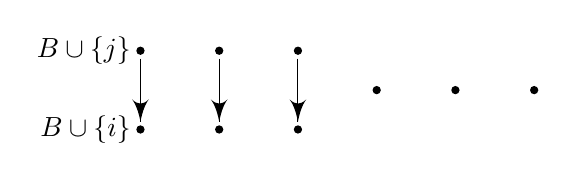
\begin{tikzpicture}
    \foreach \x in {0,1,2} {
      \node [circ] at (\x, 0) {};
      \node [circ] at (\x, -1) {};
      \draw [->] (\x, -0.1) -- (\x, -0.9) {};
    }
    \node [left] at (0, 0) {$B \cup \{j\}$};
    \node [left] at (0, -1) {$B \cup \{i\}$};
    \foreach \y in {3, 4, 5} {
      \node [circ] at (\y, -0.5) {};
    }
  \end{tikzpicture}
\end{center}
The set system $\mathcal{A}$ is some subset of all these points, we what we are doing is that we are pushing everything down when possible.

It is clear that we have $|C_{ij}(\mathcal{A})| = |\mathcal{A}|$.

\begin{lemma}
  We have
  \[
    \partial C_{ij}(\mathcal{A}) \subseteq C_{ij}(\partial \mathcal{A}).
  \]
  In particular, $|\partial C_{ij}(\mathcal{A})| \leq |\partial \mathcal{A}|$.
\end{lemma}

\begin{proof}
  Exercise.
\end{proof}

Given $\mathcal{A} \subseteq X^{(r)}$, we say $\mathcal{A}$ is left-compressed if $c_{ij}(\mathcal{A}) = \mathcal{A}$ for all $i < j$.

Initial segments are left-compressed, but the converse is false! For example, $\{123, 124, 125, 126\}$ are left-compressed, but not an initial segment! So let's look for a more powerful compressions.

For $U, V \in X^{(s)}$ with $U \cap V = \emptyset$, we define a $(U, V)$-compression as follows: for $A \subseteq X$, we define
\[
  C_{UV}(A) = 
  \begin{cases}
    (A \setminus V) \cup U & A \cap (U \cup V) = V\\
    A & \text{otherwise}
  \end{cases}
\]
Again, for $\mathcal{A} \subseteq X^{(r)}$, we can define
\[
  C_{UV}(\mathcal{A}) = \{C_{UV}(A) : A \in \mathcal{A}\} \cup \{A \in \mathcal{A}: C_{UV}(A) \in \mathcal{A}\}.
\]
Again, $\mathcal{A}$ is $(U, V)$-compressed if $C_{UV}(\mathcal{A}) = \mathcal{A}$.

\begin{lemma}
  Let $\mathcal{A} \subseteq X^{(r)}$ and $U, V \in X^{(s)}$, $U \cap V = \emptyset$. Suppose for all $u \in U$, there exists $v$ such that $\mathcal{A}$ is $(U \setminus \{u\}, V \setminus \{v\})$-compressed. Then
  \[
    \partial C_{UV} (\mathcal{A}) \subseteq C_{UV}(\partial A).
  \]
\end{lemma}

\begin{lemma}
  $\mathcal{A} \subseteq X^{(r)}$ is an initial segment of $X^{(r)}$ in colex if and only if it is $(U, V)$-compressed for all $U, V$ disjoint with $|U| = |V|$ and $\max V > \max U$.
\end{lemma}

\begin{proof}
  $\Rightarrow$ is clear. Suppose $\mathcal{A}$ is $(U, V)$ compressed for all such $U, V$. If $\mathcal{A}$ is not an initial segment, then there exists $B \in \mathcal{A}$ and $C \not \in \mathcal{A}$ such that $C < B$. Then $\mathcal{A}$ is not $(C \setminus B, B \setminus C)$-compressed. A contradiction.
\end{proof}

\begin{lemma}
  Given $\mathcal{A} \in X^{(r)}$, there exists $\mathcal{B} \subseteq X^{(r)}$ such that $B$ is $(U, V)$-compressed for all $|U| = |V|$, $U \cap B= \emptyset$, $\max V > \max U$, and moreover
  \[
    |\mathcal{B}| = |\mathcal{A}|, |\partial \mathcal{B}| \leq |\partial \mathcal{A}|.\tag{$*$}
  \]
\end{lemma}

\begin{proof}
  Let $\mathcal{B}$ be such that
  \[
    \sum_{B \in \mathcal{B}} \sum_{i \in B} 2^i
  \]
  is minimal among those $\mathcal{B}$'s that satisfy $(*)$. We claim that this $\mathcal{B}$ will do. Indeed, if there exists $(U, V)$ such that $|U| = |V|$, $\max V > \max U$ and $C_{UV}(\mathcal{B}) \not \mathcal{B}$, then pick such a pair with $|U|$ minimal. Then apply a $(U, V)$-compression, which is valid since given any $u \in U$we can pick any $v \in V$ that is not $\max V$ to satisfy the requirements of the previous lemma. This decreases the sum. This is a contradiction.
\end{proof}

From these, we know that
\begin{thm}[Kruskal 1963, Katona 1968]
  Let $\mathcal{A} \subseteq X^{(r)}$, and let $\mathcal{C} \subseteq X^{(r)}$ be the initial segment with $|\mathcal{C}| = |\mathcal{A}|$. Then
  \[
    |\partial \mathcal{A}| \geq |\partial \mathcal{C}|.
  \]
\end{thm}

We can now define the \term{shadow function}
\[
  \partial^{(r)}(m) = \min\{|\partial \mathcal{A}| : \mathcal{A} \subseteq X^{(r)}, |\mathcal{A}| = m\}.
\]
This does not depend on the size of $X$ as long as $X$ is large enough to acommodate $m$ sets, i.e.\ $\binom{n}{r} \geq m$. We know that
\[
  \partial^{(r)}\left( \sum_{i = s}^r \binom{m_i}{i}\right) = \sum_{i = s}^r \binom{m_i}{i - 1},
\]
and we also know that every $m$ can be expressed in the form $\sum_{i = s}^r \binom{m_i}{i}$ for some unique chocies of $m_i$.

This result is particularly nice for $m = \binom{n}{r}$:
\[
  \partial^{(r)}\left(\binom{n}{r}\right) = \binom{n}{r - 1}.
\]
\begin{thm}[Lov\a'ss, 1979] % check this
  If $\mathcal{A} \subseteq X^{(r)}$ with $|\mathcal{A}| = \binom{x}{r}$ for $x \geq 1, x \in \R$, then
  \[
    |\partial \mathcal{A}| \geq \binom{x}{r - 1}.
  \]
  This is best possible if $x$ is an integer.
\end{thm}
\printindex
\end{document}
